\chapter{Theoretische Grundlagen}
\label{ch:chapter02}

In diesem Kapitel werden die wesentlichen theoretischen Grundlagen vorgestellt, die für das Verständnis dieser Arbeit notwendig sind. Zunächst werden die grundlegenden Konzepte von Cloud Computing und Microservices-Architektur erläutert, um die Ausgangslage verteilter Systeme zu verstehen. Anschließend werden Serverless-Computing und \ac{FaaS} erläutert, wobei \ac{AWS} als konkrete Plattform und \ac{AWS} Lambda als konkrete \ac{FaaS}-Implementierung im Mittelpunkt stehen. Anschließend werden Observability, Distributed Tracing, OpenTelemetry und die \ac{ADOT} vorgestellt. Abschließend werden Cloud-Ressourcen und -Dienste von \ac{AWS} wie z. B. \ac{AWS} CloudWatch, \ac{AWS} X‑Ray beschrieben, die für die Implementierung und Evaluierung der in dieser Arbeit vorgeschlagenen Lösung relevant sind.

\section{Cloud Computing}
\label{sec:cloud}

Cloud Computing ermöglicht den bedarfsgerechten Zugriff auf IT-Ressourcen über das Internet, ohne dass der Nutzer die zugrunde liegende Hardware selbst verwalten muss~\cite{Mell2011NIST}. Für diese Arbeit ist vor allem die nutzungsbasierte Abrechnung (Pay‑per‑Use) relevant, da sie die wirtschaftliche Bedeutung des Tracing-Overheads unterstreicht – jede zusätzliche Millisekunde Laufzeit wirkt sich direkt auf die Kosten aus.
Cloud Computing zeichnet sich durch fünf wesentliche Merkmale aus, die Huawei Technologies Co., Ltd. in \emph{Cloud Computing Technology} wie folgt beschreibt~\cite{Huawei2023CloudComputing}:
\begin{itemize}
    \item \textbf{Bedarfsgerechte Selbstbedienung (On-Demand Self-Service):} Nutzer können Rechenressourcen eigenständig und ohne menschliche Interaktion mit dem Anbieter beziehen.
    \item \textbf{Umfassender Netzwerkzugang (Extensive Network Access):} Alle Cloud-Dienste sind über das Netzwerk (meist Internet) standardisiert und von verschiedenen Endgeräten erreichbar.
    \item \textbf{Ressourcenbündelung (Resource Pooling):} Physische und virtuelle Ressourcen werden in einen gemeinsamen Pool zusammengefasst und dynamisch an mehrere Nutzer verteilt.
    \item \textbf{Schnelle elastische Skalierung (Fast and Elastic Scaling):} Ressourcen können je nach Bedarf automatisch oder manuell vergrößert oder verkleinert werden.
    \item \textbf{Messbare Nutzung (Measurable Services):} Die Nutzung wird erfasst, überwacht und abgerechnet – Grundlage für Pay‑per‑Use-Modelle.
\end{itemize}

Cloud-Dienste werden üblicherweise in drei Servicemodelle unterteilt.\\ \ac{IaaS}, \ac{PaaS} und \ac{SaaS}.  
Da für diese Arbeit nur ein grundlegendes Verständnis von \ac{PaaS} relevant ist, wird das Modell kurz erläutert. 
\emph{Platform as a Service} stellt eine komplette Entwicklungsumgebung bereit, die die technische Infrastruktur abstrahiert. 
Nutzer entwickeln und betreiben ihre Anwendungen direkt auf dieser Plattform, ohne sich um Betriebssysteme, Skalierung oder Wartung 
kümmern zu müssen~\cite{Huawei2023CloudComputing}. 
Eine besondere Ausprägung von PaaS ist das \ac{FaaS}-Modell. 
Die in dieser Arbeit untersuchten AWS-Lambda-Funktionen folgen genau diesem FaaS-Modell 
(siehe Abschnitt~\ref{sec:serverless}).

\section{Microservices und Event-Driven Architecture}
\label{sec:microservices-eda}

Microservices und \ac{EDA} sind zwei eng verbundene Architekturstile moderner Cloud-nativer Systeme~\cite{Fowler2024Microservices,Katzer2024Serverless}.  
Während Microservices eine Anwendung in kleine, unabhängig bereitstellbare Dienste unterteilen~\cite{Fowler2024Microservices}, definiert \ac{EDA} ein asynchrones Kommunikationsmuster über Ereignisse~\cite{AWSEventDrivenArchitecture}.  
Für diese Arbeit ist das Zusammenspiel beider Konzepte zentral, weil \ac{FaaS} typischerweise als Event-Consumer und oder Event-Producer in einer ereignisgesteuerten Microservices-Umgebung agieren~\cite{AWSLambdaDocs}.

\subsection{Microservices}
Microservices sind unabhängige, lose gekoppelte Dienste, die jeweils einen eigenen Bereich der Geschäftslogik einer Anwendung abdecken. 
Die zentralen Merkmale von Microservices sind, dass sie in unterschiedlichen Programmiersprachen implementiert, separat getestet, gewartet, skaliert und deployed werden können, ohne
dass die anderen Dienste beeinflusst werden~\cite{Fowler2024Microservices}. Dieser Architekturstil ist relevant, 
da die Serverless-Technologien und die FaaS-Plattformen speziell für die Entwicklung von Microservices konzipiert sind (siehe Abschnitt~\ref{sec:serverless}). 
Zudem sind die 5 Microbenchmarks typische Beispiele für Microservices (siehe Abschnitt~\ref{subsec:lambda-benchmarks}).

\begin{figure}[H]
 \centering
 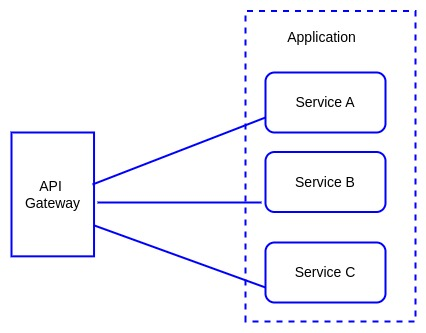
\includegraphics[width=0.5\textwidth]{gfx/examples/microservices.jpg}
 \caption{Microservices}
 \label{fig:chapter02:EDA}
\end{figure}

Abbildung~\ref{fig:chapter02:EDA} stellt das obige Konzept der Microservices visuell dar.

\subsection{Event-Driven Architecture}
In einer \ac{EDA} kommunizieren Dienste nicht synchron über \ac{HTTP}-Anfragen, sondern asynchron über Ereignisse~\cite{AWSEventDrivenArchitecture}.
Der Gedanke hinter \ac{EDA} ist, dass Dienste lose gekoppelt sind und dass sie auf Ereignisse reagieren, anstatt direkt miteinander zu kommunizieren. 
Ein \textit{Event Producer} sendet ein Ereignis an einen \textit{Event Broker}. Ein Event Broker ist ein Vermittler, der die Ereignisse 
empfängt, speichert und an die entsprechenden Event Consumer weiterleitet. Beispiele für Event Broker sind AWS \ac{SNS}, \ac{SQS} usw. oder 
auch platforminterne Event-Puffer, die Events nur kurzfristig speichern, bis sie von den \textit{Event Consumern} abgeholt werden~\cite{AWSEventDrivenArchitecture,AzureEventDrivenArchitecture}. 
Event Consumer sind Dienste, die auf bestimmte Ereignisse reagieren, indem sie eine Aktion ausführen (z. B. eine Lambda-Funktion ausführen, eine Datenbank aktualisieren).
Den Prozess, bei dem ein Event Producer ein Ereignis an einen Event Broker sendet und der Event Broker dieses Ereignis an die entsprechenden Event Consumer weiterleitet, bezeichnet man
als \textit{Event Ingestion} oder auch \textit{Event Processing}.
Diese Entkopplung erhöht die Ausfallsicherheit und ist die Grundlage für die ereignisgesteuerte Ausführung von 
AWS-Lambda-Funktionen~\cite{Rocha2021Practical}.

\begin{figure}[H]
 \centering
 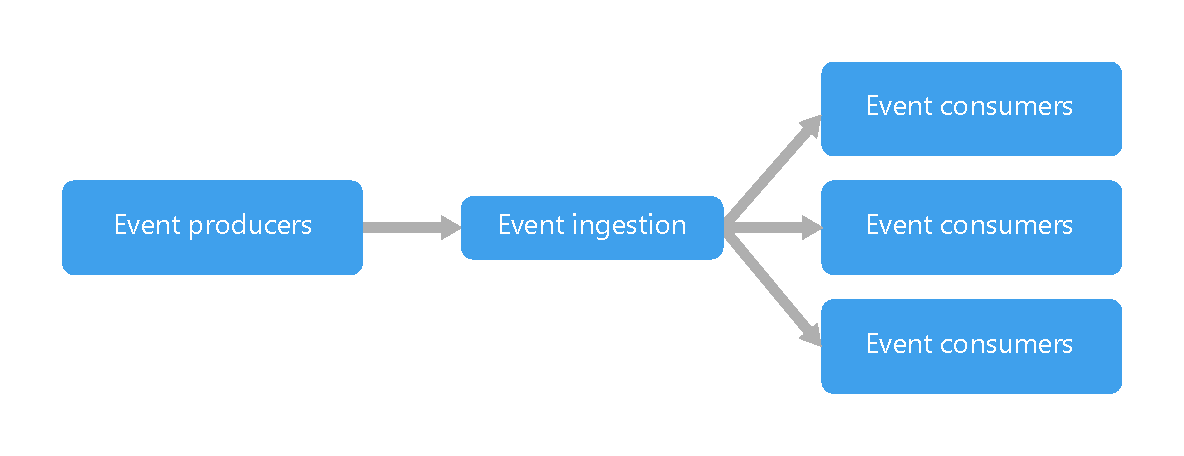
\includegraphics[width=0.9\textwidth]{gfx/examples/eda-azure.pdf}
 \caption{EDA-Struktur~\cite{AzureEventDrivenArchitecture}}
 \label{fig:chapter02:monolith-vs-microservices}
\end{figure}
Abbildung~\ref{fig:chapter02:monolith-vs-microservices} stellt das oben beschriebene Konzept der Event-Driven Architecture visuell dar.

\subsection{Zusammenspiel von Microservices und EDA}
Die Kombination von Microservices und \ac{EDA} adressiert zentrale Herausforderungen verteilter Systeme. 
Durch lose Kopplung müssen Dienste keine Kenntnis voneinander haben. Ein Producer publiziert ein Event, ohne die Consumer zu kennen. 
Fällt ein Consumer aus, bleibt der Producer funktionsfähig, was die Ausfallsicherheit erhöht~\cite{Rocha2021Practical}.  
Für diese Arbeit ist dieses Zusammenspiel fundamental, da die AWS-Lambda-Funktionen sowohl Events konsumieren als auch produzieren 
können~\cite{AWSLambdaDocs}. Damit sind sie in ihrem Kern ereignisgesteuerte Microservices.

\section{Serverless-Computing und Function as a Service}
\label{sec:serverless}

Serverless-Computing ist ein Cloud-Ausführungsmodell, bei dem der Anbieter die gesamte Serverinfrastruktur verwaltet und der Entwickler sich nur auf die Anwendungslogik konzentriert. Der Begriff „serverless“ ist irreführend, da weiterhin Server im Hintergrund laufen, diese aber vollständig abstrahiert sind~\cite{IBMFaaS}.  
Für diese Arbeit ist das \ac{FaaS}-Modell zentral, weil es als die am weitesten verbreitete Form von Serverless gilt~\cite{ServerlessAWSLambda}.

\subsection{FaaS als zentrale Ausprägung}
Im Zentrum von Serverless-Computing steht das \ac{FaaS}-Modell.
Dabei wird die Geschäftslogik einer Anwendung in kleine, unabhängige und zustandslose Funktionen unterteilt, die durch Ereignisse (z. B. \ac{HTTP}-Anfragen, Datenbankänderungen, Datei-Uploads usw.) ausgelöst werden~\cite{IBMFaaS}. 
Jede Funktion ist eine eigenständige Einheit (\ac{FaaS}-Instanz).
Die wichtigsten Eigenschaften von \ac{FaaS}, die für die Messung relevant sind, sind:
\begin{itemize}
    \item \textbf{Ereignisgesteuerte Ausführung:} Funktionen werden nur bei Bedarf aktiviert und verbrauchen im Leerlauf keine Ressourcen. Das beeinflusst die Messung sowohl von Warmstarts als auch von Kaltstarts für alle zu messenden Metriken (siehe Kapitel \ref{ch:chapter04}).
    \item \textbf{Automatische Skalierung:} Die Plattform skaliert die Anzahl der Instanzen dynamisch, was die Messung bei steigender Last relevant macht und eine präzise Dokumentation erfordert.
    \item \textbf{Pay-per-Use-Abrechnung:} Abgerechnet wird nach Ausführungszeit und Speicherzuweisung. Dadurch wirkt sich jeder durch Tracing verursachte Overhead direkt auf die Kosten aus.
\end{itemize}
FaaS-Plattformen setzen intern auf Container-Technologie. Bei einem Aufruf wird die Funktion in einen vorkonfigurierten Container geladen und ausgeführt. Nach Abschluss bleibt der Container kurz erhalten (Warmstart) oder wird freigegeben (Kaltstart)~\cite{ServerlessAWSLambda}.
Abbildung~\ref{fig:chapter02:faas} zeigt das Prinzip von FaaS. Entwickler stellen nur den Code bereit, die Plattform kümmert sich um die Ausführung, Skalierung, Verwaltung usw. 
Im Gegensatz zu \ac{IaaS}, bei dem der Nutzer virtuelle Maschinen selbst verwaltet, oder \ac{PaaS}, das eine Plattform für vollständige Anwendungen bereitstellt, beschränkt sich \ac{FaaS} auf einzelne Funktionen und skaliert automatisch. \ac{SaaS} liefert fertige Anwendungen, während FaaS nur die Ausführungsumgebung zur Verfügung stellt.
\begin{figure}[H]
 \centering
 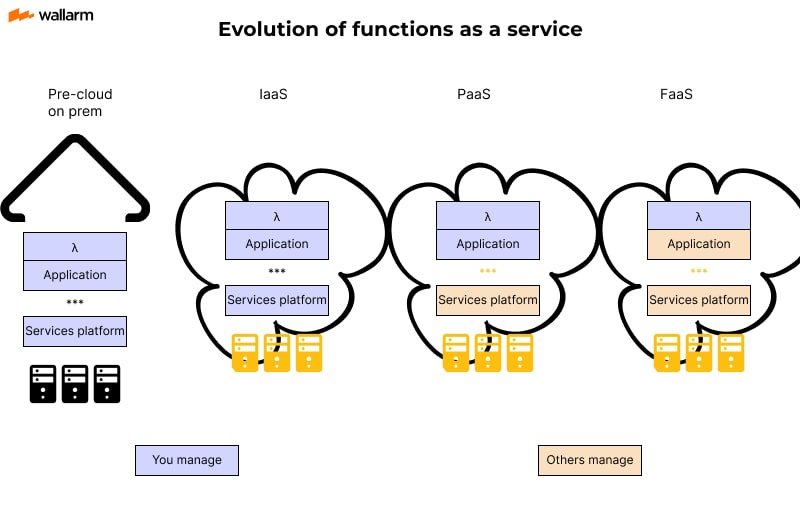
\includegraphics[width=1.0\textwidth]{gfx/examples/FaaS.jpg}
 \caption{Function as a Service \href{https://www.wallarm.com/what/what-is-faas-function-as-a-service}{[\cite{WallarmFaaS}]}}
 \label{fig:chapter02:faas}
\end{figure}
\subsection{Vorteile und Herausforderungen im Kontext dieser Arbeit}

Serverless-Anwendungen reduzieren den operativen Aufwand und ermöglichen eine kosteneffiziente 
Skalierung. Allerdings gibt es spezifische Herausforderungen, die für die Messung relevant sind. 
Die größte Herausforderung ist die Initialisierungsverzögerung (Cold Start), die bei der ersten 
Ausführung einer Funktion auftritt, wenn die Plattform eine neue Instanz bereitstellen muss. 
Eine andere Herausforderung ist die Bindung an einen bestimmten Anbieter (Vendor Lock-in), 
da die Funktionen oft auf spezifische Dienste und APIs des Anbieters angewiesen sind.

\section{AWS Lambda als konkrete FaaS-Plattform}
\label{sec:aws-lambda}

AWS Lambda ist der von Amazon Web Services bereitgestellte FaaS-Dienst und gilt als einer der beliebtesten Vertreter dieser Kategorie~\cite{ServerlessAWSLambda}. Er bildet die Plattform für alle in dieser Arbeit durchgeführten Experimente.

\subsection{Grundlegende Funktionsweise}

Eine Lambda-Funktion ist ein Code-Block, der durch ein Ereignis (z. B. eine \ac{HTTP}-Anfrage, ein Datei-Upload) ausgelöst wird. 
Die Funktion besitzt genau einen \textit{Handler}, der die Ereignisdaten verarbeitet. Bei der Bereitstellung werden Code und 
Abhängigkeiten als ZIP- oder Container-Image gepackt~\cite{AWSLambdaBasics}.  
Lambda erstellt bei Bedarf eine isolierte Ausführungsumgebung (\textit{execution environment}), die 
nach der Ausführung kurz beibehalten wird, um nachfolgende Aufrufe schneller zu bedienen (Warmstart)~\cite{AWSLambdaBasics}.
Der Aufruf kann direkt über die Konsole, CLI oder SDKs erfolgen oder im produktiven Einsatz typisch durch andere 
AWS-Dienste (Trigger). Lambda-Funktionen können von vielen AWS-Diensten wie S3, DynamoDB, API Gateway oder
 SQS ausgelöst werden~\cite{AWSLambdaServices}.

\subsection{Lambda Layers}
\label{subsec:lambda-layers}

Ein \textit{Layer} ist ein ZIP-Archiv, das Bibliotheken oder Konfigurationen kapselt und mehreren Funktionen gemeinsam zur Verfügung gestellt werden kann~\cite{AWSLambdaLayers}. Für diese Arbeit ist der von AWS bereitgestellte Layer für die \ac{ADOT} zentral, der die OpenTelemetry-Abhängigkeiten enthält und eine einfache, performante Instrumentierung ermöglicht (siehe Abschnitt~\ref{sec:adot}).

\begin{figure}[H]
 \centering
 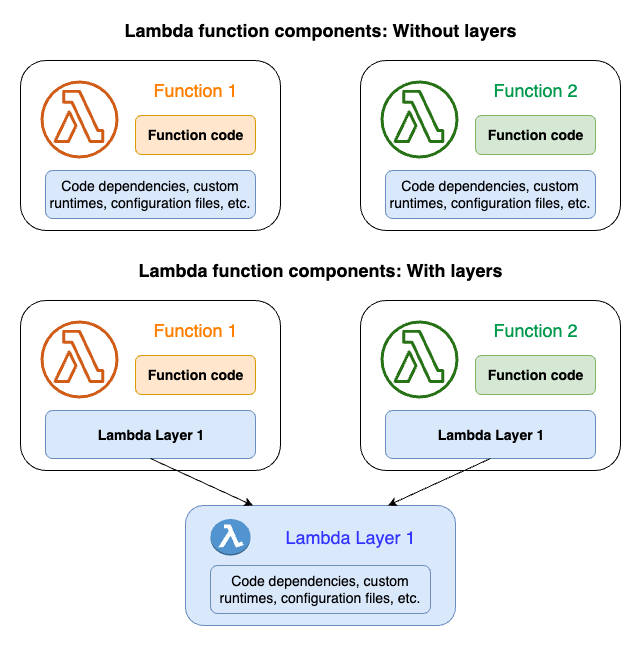
\includegraphics[width=1.0\textwidth]{gfx/examples/lambda-layers-diagram.png}
 \caption{AWS Lambda Layers~\cite{AWSLambdaLayers}}
 \label{fig:chapter02:aws_lambda_layers}
\end{figure}
Abbildung~\ref{fig:chapter02:aws_lambda_layers} zeigt schematisch die Funktionsweise und die konkreten Vorteile von Lambda Layers.


\subsection{Häufigste Anwendungsfälle von AWS Lambda}
\label{subsec:lambda-benchmarks}

\begin{figure}[H]
 \centering
 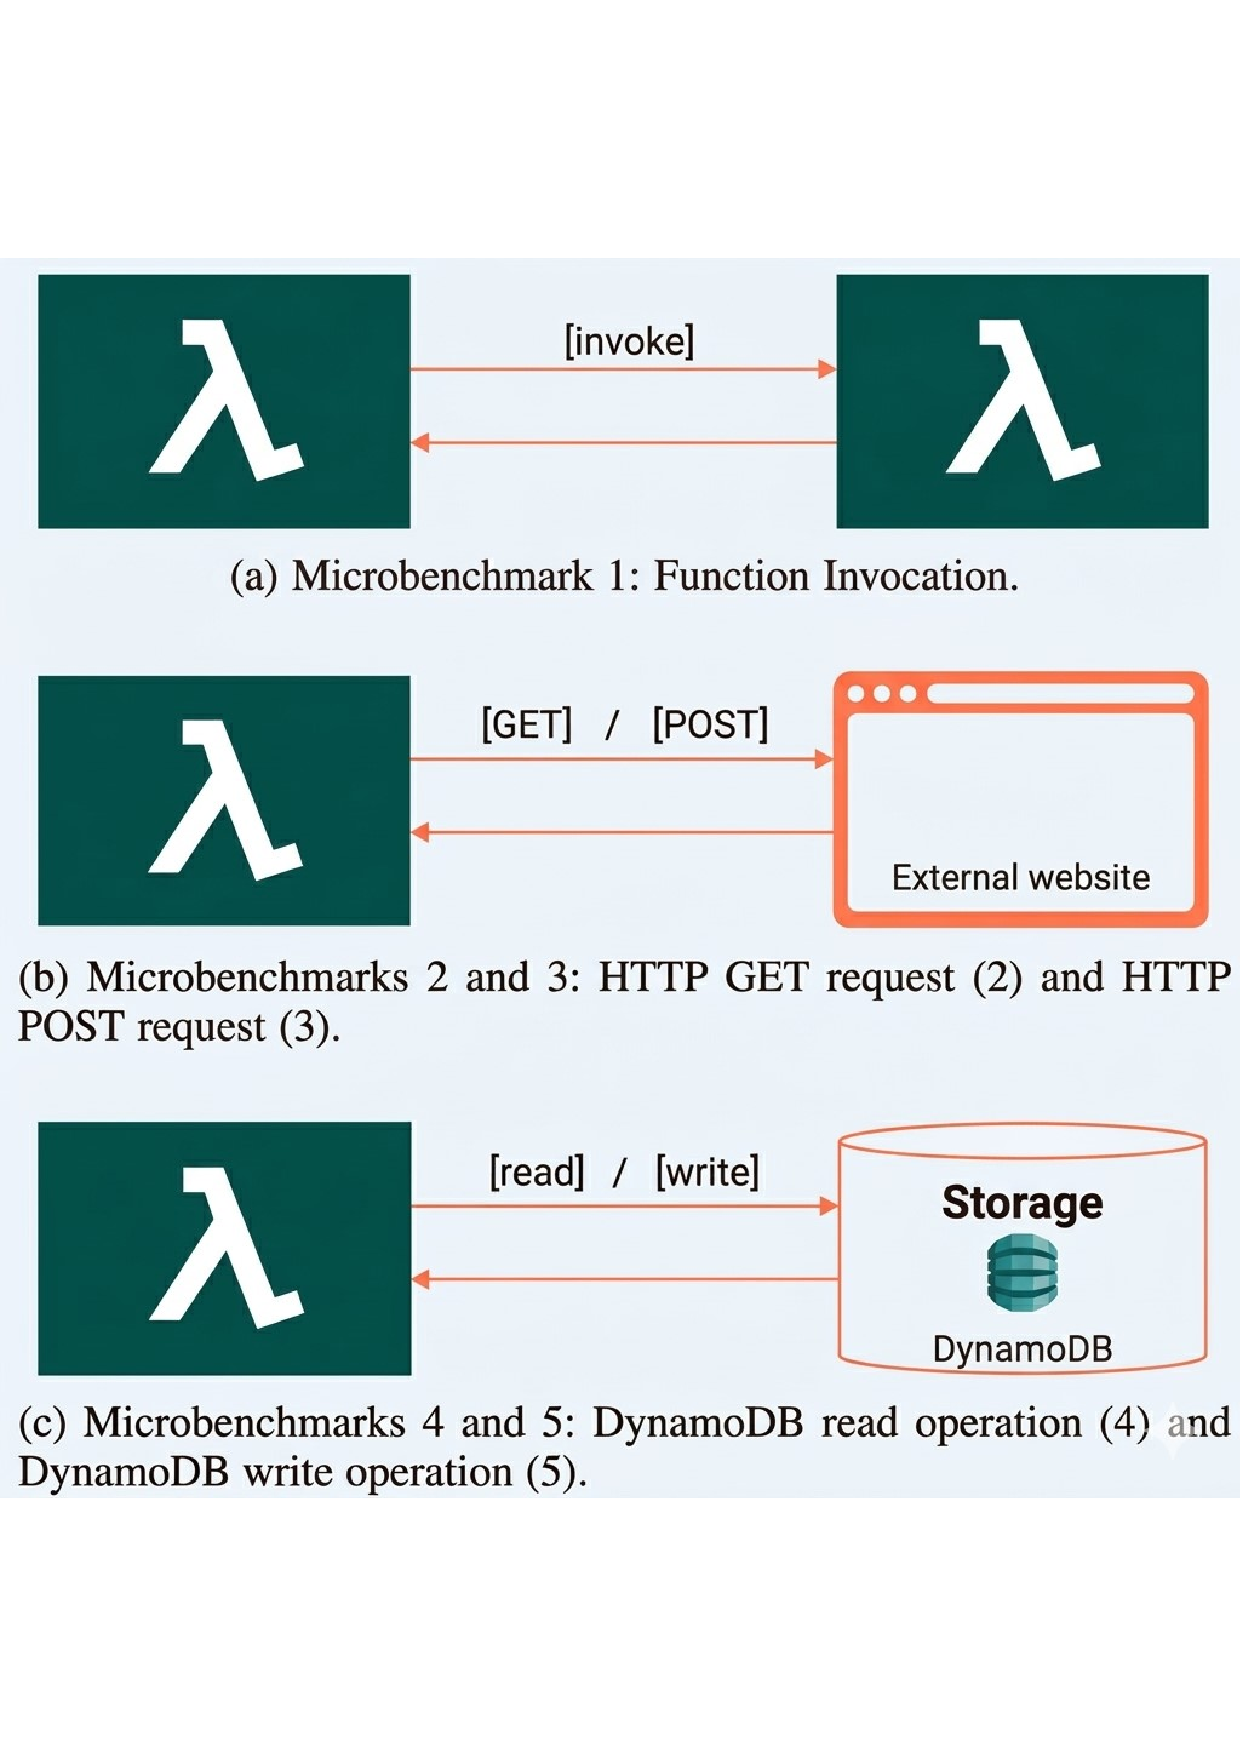
\includegraphics[width=0.6\textwidth]{gfx/examples/Microbenchmarks.pdf}
 \caption{Häufigste Anwendungsfälle von AWS Lambda.}
 \label{fig:chapter02:aws_lambda_use_cases}
\end{figure}
Die in Abbildung~\ref{fig:chapter02:aws_lambda_use_cases} dargestellten fünf Microbenchmarks repräsentieren die häufigsten Interaktionsmuster von AWS-Lambda-Funktionen~\cite{Winzinger2021DataFlow}:
\begin{enumerate}
    \item Eine Lambda-Funktion ruft eine weitere Lambda-Funktion auf (Lambdaverkettung).
    \item Eine Lambda-Funktion sendet eine HTTP-GET-Anfrage an eine externe API.
    \item Eine Lambda-Funktion sendet eine HTTP-POST-Anfrage an eine externe API.
    \item Eine Lambda-Funktion führt eine Leseoperation aus einer DynamoDB-Tabelle durch.
    \item Eine Lambda-Funktion führt eine Schreiboperation in eine DynamoDB-Tabelle durch.
\end{enumerate}
Diese fünf Szenarien basieren auf einer umfassenden Analyse (siehe~\cite{Winzinger2021DataFlow}) und bilden die Grundlage für die experimentelle Evaluation in Kapitel~\ref{ch:chapter04} und Kapitel~\ref{ch:chapter05}. Für jedes Szenario wird jeweils eine instrumentierte und eine nicht-instrumentierte Version der Funktion in den drei Sprachen Java, Python und Node.js implementiert.

\section{Observability in verteilten Systemen}
\label{sec:observability}

Observability beschreibt die Fähigkeit, den internen Zustand eines Systems allein durch seine externen Ausgaben 
(Logs, Metriken, Traces) zu verstehen. In verteilten, Cloud-nativen Umgebungen ist dies eine Grundvoraussetzung für 
Fehlerdiagnose und Performance-Optimierung~\cite{Hausenblas2024Cloud}.

\begin{figure}[H]
 \centering
 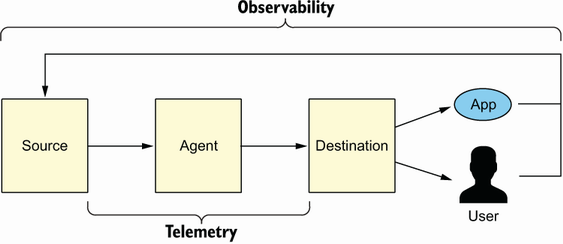
\includegraphics[width=0.9\textwidth]{gfx/examples/observability_struktur.png}
 \caption{Zentrale Komponenten von Observability~\cite{Hausenblas2024Cloud}}
 \label{fig:chapter02:observability}
\end{figure}
Abbildung~\ref{fig:chapter02:observability} stellt die zentralen Komponenten der Observability dar. 
Das beobachtete \textit{System} (System under Observation) umfasst die gesamte cloud-native Plattform samt Anwendungen, 
von deren \textit{Sources} also Quellen (wie Microservices oder Datenbanken) durch Instrumentierung beobachtbare \textit{Signals} 
(Signale) wie Logs, Metriken und Traces ausgehen. Diese Daten werden von \textit{Agents} (Agenten) gesammelt, verarbeitet 
und an verschiedene \textit{Destinations} (Ziele) weitergeleitet, um sie für Dashboards, Alarme oder Analysen zu nutzen. 
Dieser gesamte Kreislauf vom Erfassen über das Routing bis zum Speichern der Daten wird als \textit{Telemetry} (Telemetrie) bezeichnet.

\subsection{Die drei Säulen der Observability}
Die drei zentralen Signaltypen, die auch als \glqq \emph{die drei Säulen der Observability}\grqq{} bezeichnet werden, sind 
\emph{Logs}, \emph{Metriken} und \emph{Traces}. 

\emph{Logs} sind detaillierte, zeitgestempelte Aufzeichnungen von Ereignissen. 

\emph{Metriken} sind numerische Messwerte eines Systems, die sich für visuelle Dashboards und Alarme eignen. 

\emph{Traces} ermöglichen die Nachverfolgung einer Anfrage mittels context-propagation durch verschiedene Dienste hinweg.
Erst die Kombination aller drei Säulen ermöglicht ein vollständiges Bild des Systemverhaltens~\cite{Hausenblas2024Cloud}. 
Für diese Arbeit sind \textit{Metriken} (Laufzeit, Speicher, Kaltstartdauer), \textit{Logs} (zur Extraktion von Metriken und Fehleranalyse) und \textit{Traces} (zur Validierung der Instrumentierung) relevant.

\section{OpenTelemetry}
\label{sec:otel}
OpenTelemetry ist ein Open-Source-Standard, der die Erfassung von Telemetriedaten vereinheitlicht und eine gemeinsame API bereitstellt, 
sodass Anwendungen nicht für jedes Backend neu instrumentiert werden müssen. Ziel ist es, eine einheitliche Bibliothek für Logs, 
Metriken und Traces zu schaffen und Vendor-Lock-in zu vermeiden~\cite{OpenTelemetryInstrumentation,OpenTelemetryWhatIs}.


\subsection{Kernkomponenten und Architektur}
Die OpenTelemetry-Architektur besteht aus mehreren modularen Komponenten~\cite{OpenTelemetryComponents,OpenTelemetryInstrumentation}:
\begin{itemize}
    \item \textbf{API und SDK:} Die \ac{API} definiert, wie Telemetriedaten erzeugt werden; das \ac{SDK} bietet konkrete Implementierungen und Konfigurationsmöglichkeiten (z. B. Sampling, Export). Entwickler können zwischen manueller (codebasierter) und automatischer (Zero-Code-)Instrumentierung wählen.
    \item \textbf{Instrumentierungsbibliotheken:} Vorgefertigte Bibliotheken für gängige Frameworks (HTTP, Datenbanken), die automatisch Telemetriedaten erzeugen. Langfristig sollen alle wichtigen Bibliotheken standardmäßig beobachtbar sein.
    \item \textbf{Collector:} Eine Komponente, die Telemetriedaten empfängt, verarbeitet (filtern, anreichern, bündeln) und an ein oder mehrere Backends weiterleitet. Der Einsatz eines Collectors entkoppelt die Instrumentierung vom Backend und bietet zentrale Kontrollmöglichkeiten. In dieser Arbeit wird jedoch kein separater Collector eingesetzt. Die Daten werden direkt über den AWS-spezifischen ADOT-Layer an AWS-X-Ray exportiert.
    \item \textbf{Exporter und Propagators:} Exporter senden die Daten an ein Backend (hier AWS X-Ray), Propagators übertragen Kontextinformationen (z. B. Trace-IDs) zwischen Diensten, z. B. über \ac{HTTP}-Header.
\end{itemize}

\subsection{Sampling-Strategien}
\label{subsec:sampling}
Um das Volumen der Tracing-Daten zu reduzieren, können Sampling-Strategien angewendet werden~\cite{OpenTelemetrySampling}. 
Dies entlastet die Telemetrie-Pipeline und senkt die Kosten, da weniger Daten exportiert und gespeichert werden müssen.

\paragraph{Terminologie und Grundprinzip}
Ein Trace oder Span gilt als \emph{gesampelt (sampled)}, wenn er vom Sampler ausgewählt, verarbeitet und exportiert wird; andernfalls als \emph{nicht gesampelt (not sampled)}. Sampling ist eine effektive Methode, um Observability-Kosten zu senken, insbesondere bei hohem Durchsatz~\cite{OpenTelemetrySampling}. 

\paragraph{Head Sampling}
\emph{Head Sampling} entscheidet bereits zu Beginn eines Traces, ob er aufgezeichnet wird. Die gängigste Form ist das \emph{Consistent Probability Sampling} (deterministisches Sampling), bei dem anhand der Trace-ID und einer konstanten Rate (z. B. 5\%) entschieden wird. Vorteile sind Einfachheit und Effizienz. Nachteil ist, dass die Entscheidung nicht auf dem gesamten Trace basieren kann, sodass beispielsweise Fehler-Traces nicht gezielt erfasst werden können~\cite{OpenTelemetrySampling}.

\paragraph{Tail Sampling}
\emph{Tail Sampling} trifft die Entscheidung erst nach Betrachtung aller oder der meisten Spans eines Traces. Dadurch können komplexe Bedingungen abgebildet werden, z. B. das Aufzeichnen aller fehlerhaften Traces oder solcher mit hoher Latenz. Tail Sampling ist für größere Systeme meist die richtige Wahl, ist aber aufwendiger in der Implementierung und erfordert zustandsbehaftete Komponenten~\cite{OpenTelemetrySampling}.

In manchen Systemen werden beide Strategien kombiniert, um die Vorteile beider Ansätze zu nutzen. 
Für die Messungen in dieser Arbeit wird Head Sampling mit einer Erfassungsrate von 100\% verwendet, da das Ziel ein möglichst hohes 
Volumen an Tracing-Daten ist, um die Auswirkungen auf die Performance-Metriken umfassend zu analysieren.

\subsection{AWS Distro for OpenTelemetry (ADOT)}
\label{sec:adot}
Die \ac{ADOT} ist eine von AWS unterstützte Distribution von OpenTelemetry, die für die Integration mit AWS-Diensten 
optimiert ist~\cite{ADOT}. Für AWS Lambda werden vorgefertigte \textit{Layer} bereitgestellt, die alle notwendigen 
Abhängigkeiten enthalten und die Instrumentierung ohne manuelle SDK-Einbindung ermöglichen~\cite{ADOT_Lambda}.  
In dieser Arbeit wird ausschließlich der ADOT-Lambda-Layer verwendet, um die Instrumentierung durchzuführen. 
Als Backend dient AWS X-Ray, da es nativ mit Lambda integriert ist und die gesammelten Traces in CloudWatch verfügbar macht.


\section{AWS CloudWatch}
\label{sec:cloudwatch}

Amazon CloudWatch ist der zentrale Überwachungsdienst von AWS und sammelt Metriken und Logs aus AWS-Ressourcen~\cite{AWSCloudWatchDocs}. Für diese Arbeit ist CloudWatch die primäre Quelle der Performance-Metriken der instrumentierten Lambda-Funktionen.

\subsection{Relevante Metriken}
Für jede Lambda-Funktion stellt CloudWatch automatisch Metriken im Namespace \texttt{AWS/Lambda} bereit~\cite{AWSLambdaMetrics}. Die folgenden Metriken werden in dieser Arbeit ausgewertet:
\begin{itemize}
    \item \textbf{Duration:} Ausführungsdauer in Millisekunden (Grundlage für Runtime-Overhead).
    \item \textbf{Max Memory Used:} Maximaler Speicherverbrauch in MB (Grundlage für Memory-Overhead).
    \item \textbf{Init Duration:} Dauer der Initialisierungsphase bei Kaltstarts (Grundlage für Cold-Start-Overhead).
    \item \textbf{Invocations:} Anzahl der Aufrufe (zur Validierung der Anzahl der Aufrufe).
    \item \textbf{Errors:} Anzahl der Fehler (zur Validierung der Aufrufe).
\end{itemize}

\subsection{Datenerfassung und -analyse}
CloudWatch empfängt Metriken automatisch von Lambda nach jeder Ausführung. Darüber hinaus schreibt Lambda standardmäßig Log-Nachrichten in CloudWatch Logs, aus denen die Metriken \texttt{Init Duration}, \texttt{Duration} und \texttt{Max Memory Used} extrahiert werden können~\cite{GraylogLambdaMetrics}. Für diese Arbeit werden die relevanten Metriken aus den CloudWatch Logs extrahiert und in Kapitel \ref{ch:chapter05} analysiert.

\subsection{AWS X-Ray}
\label{subsec:aws-xray}

AWS X-Ray ist der Tracing-Dienst von AWS. Er empfängt Traces von instrumentierten Anwendungen und integrierten AWS-Diensten wie Lambda~\cite{AWSXRayDocs}.  
In dieser Arbeit fungiert X-Ray als Backend für die mit OpenTelemetry erzeugten Traces. Die Verwendung von X-Ray hat den Vorteil, dass es nativ mit Lambda zusammenarbeitet und keine zusätzliche Collector-Infrastruktur erfordert~\cite{ADOT_Lambda}.  
Die gesammelten Traces werden genutzt, um zu überprüfen, ob die Instrumentierung korrekt funktioniert und ob alle Aufrufe vollständig erfasst werden. Eine detaillierte Trace-Analyse (z. B. mit X-Ray-Queries) wird aufgrund des begrenzten Budgets nicht durchgeführt~\cite{AWSXRayPricing}.

\section{Amazon DynamoDB}
\label{sec:dynamodb}

Amazon DynamoDB ist ein vollständig verwalteter, serverloser \ac{NoSQL}-Datenbankservice, der für konsistente Latenzen im einstelligen Millisekundenbereich ausgelegt ist~\cite{AWSDynamoDBDocs}.  
In dieser Arbeit wird DynamoDB in zwei der fünf Microbenchmarks verwendet - Lese- und Schreiboperationen. Diese Szenarien repräsentieren typische Datenzugriffsmuster in serverlosen Anwendungen und ermöglichen die Messung des durch OpenTelemetry verursachten Overheads bei Datenbankoperationen.